\section{Two exits and continuous operation}
\label{sec:routes}
\begin{figure}[H]\centering
\begin{minipage}{0.49\linewidth}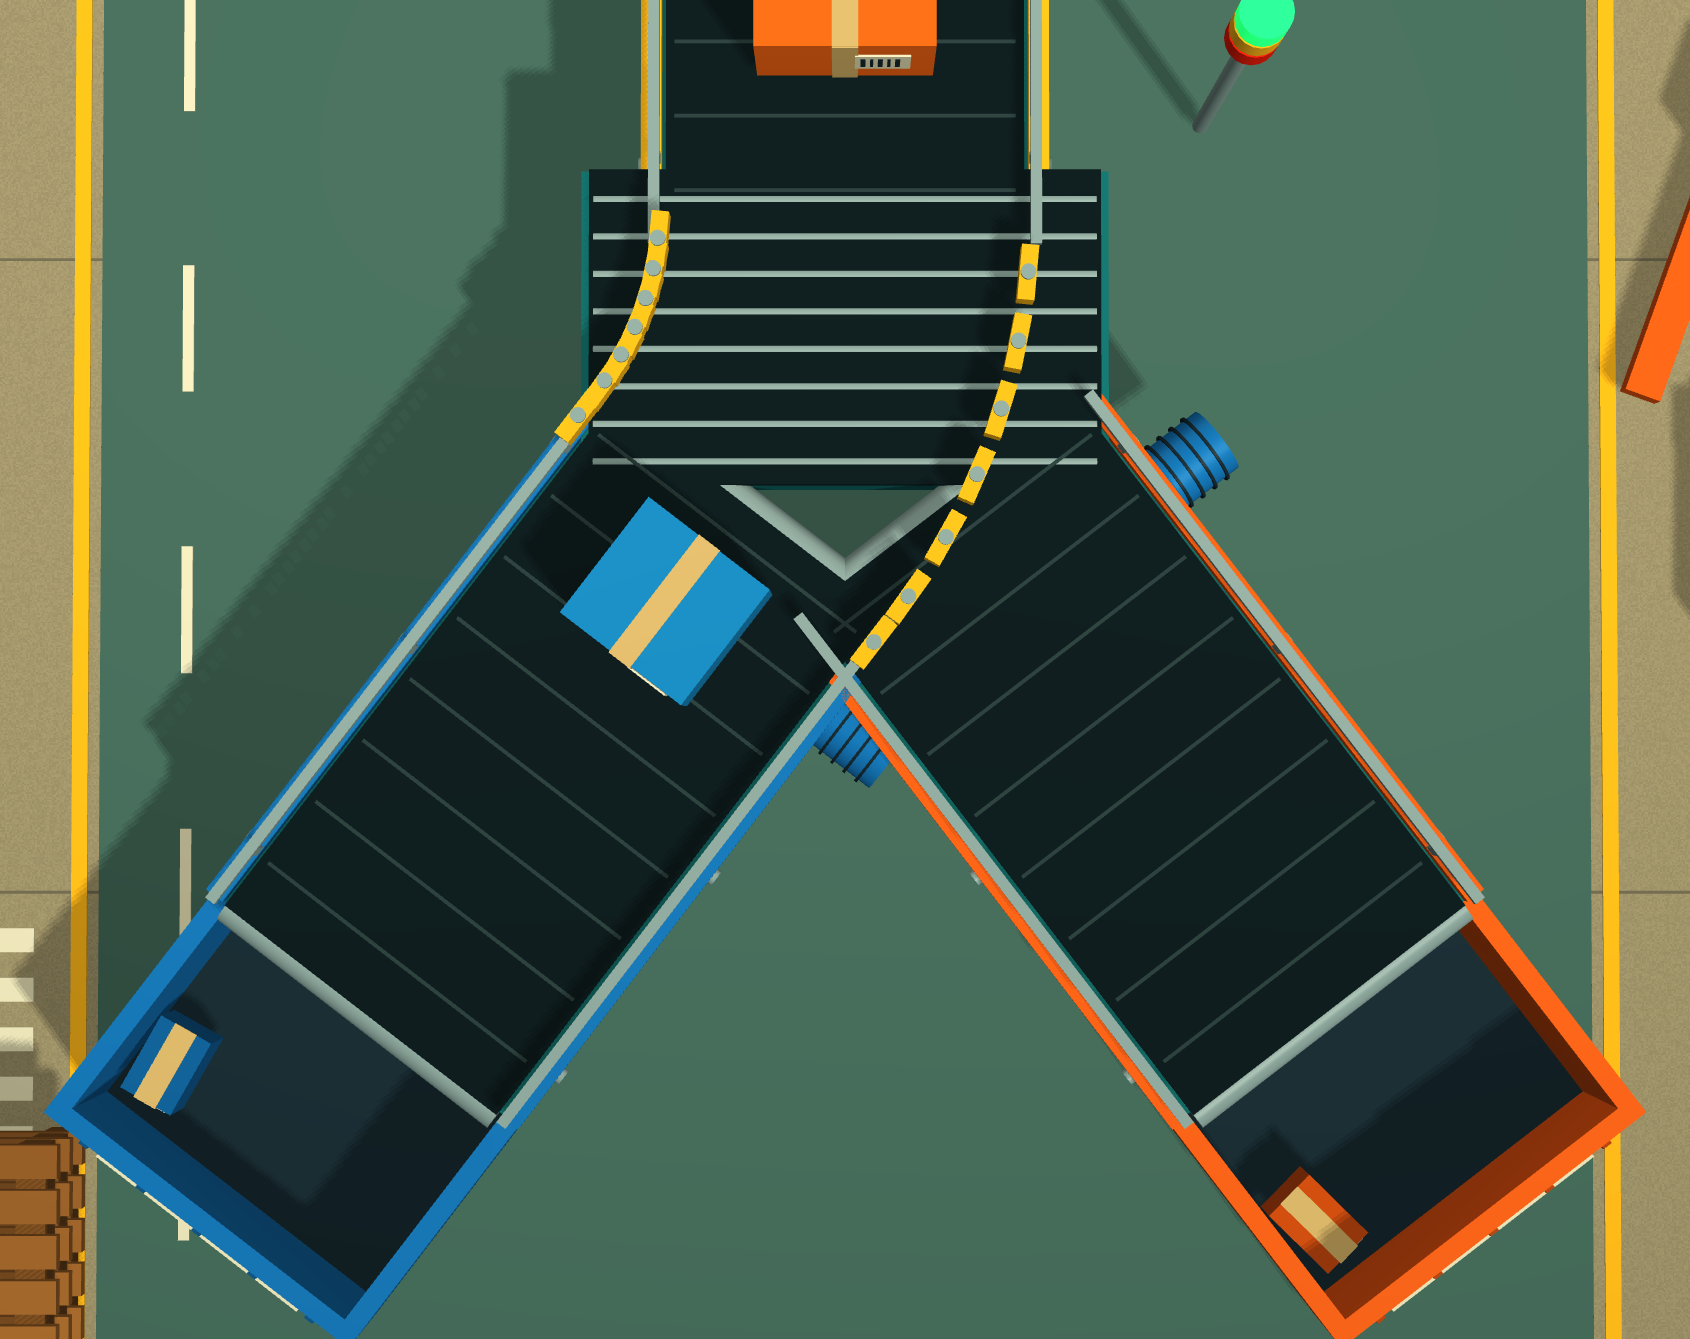
\includegraphics[width=\linewidth]{assets/gate_left_crop.png}\par\small\textbf{A. 10.20 s:} blue parcel on the left route; gate $-37.5^\circ$.\end{minipage}\hfill
\begin{minipage}{0.49\linewidth}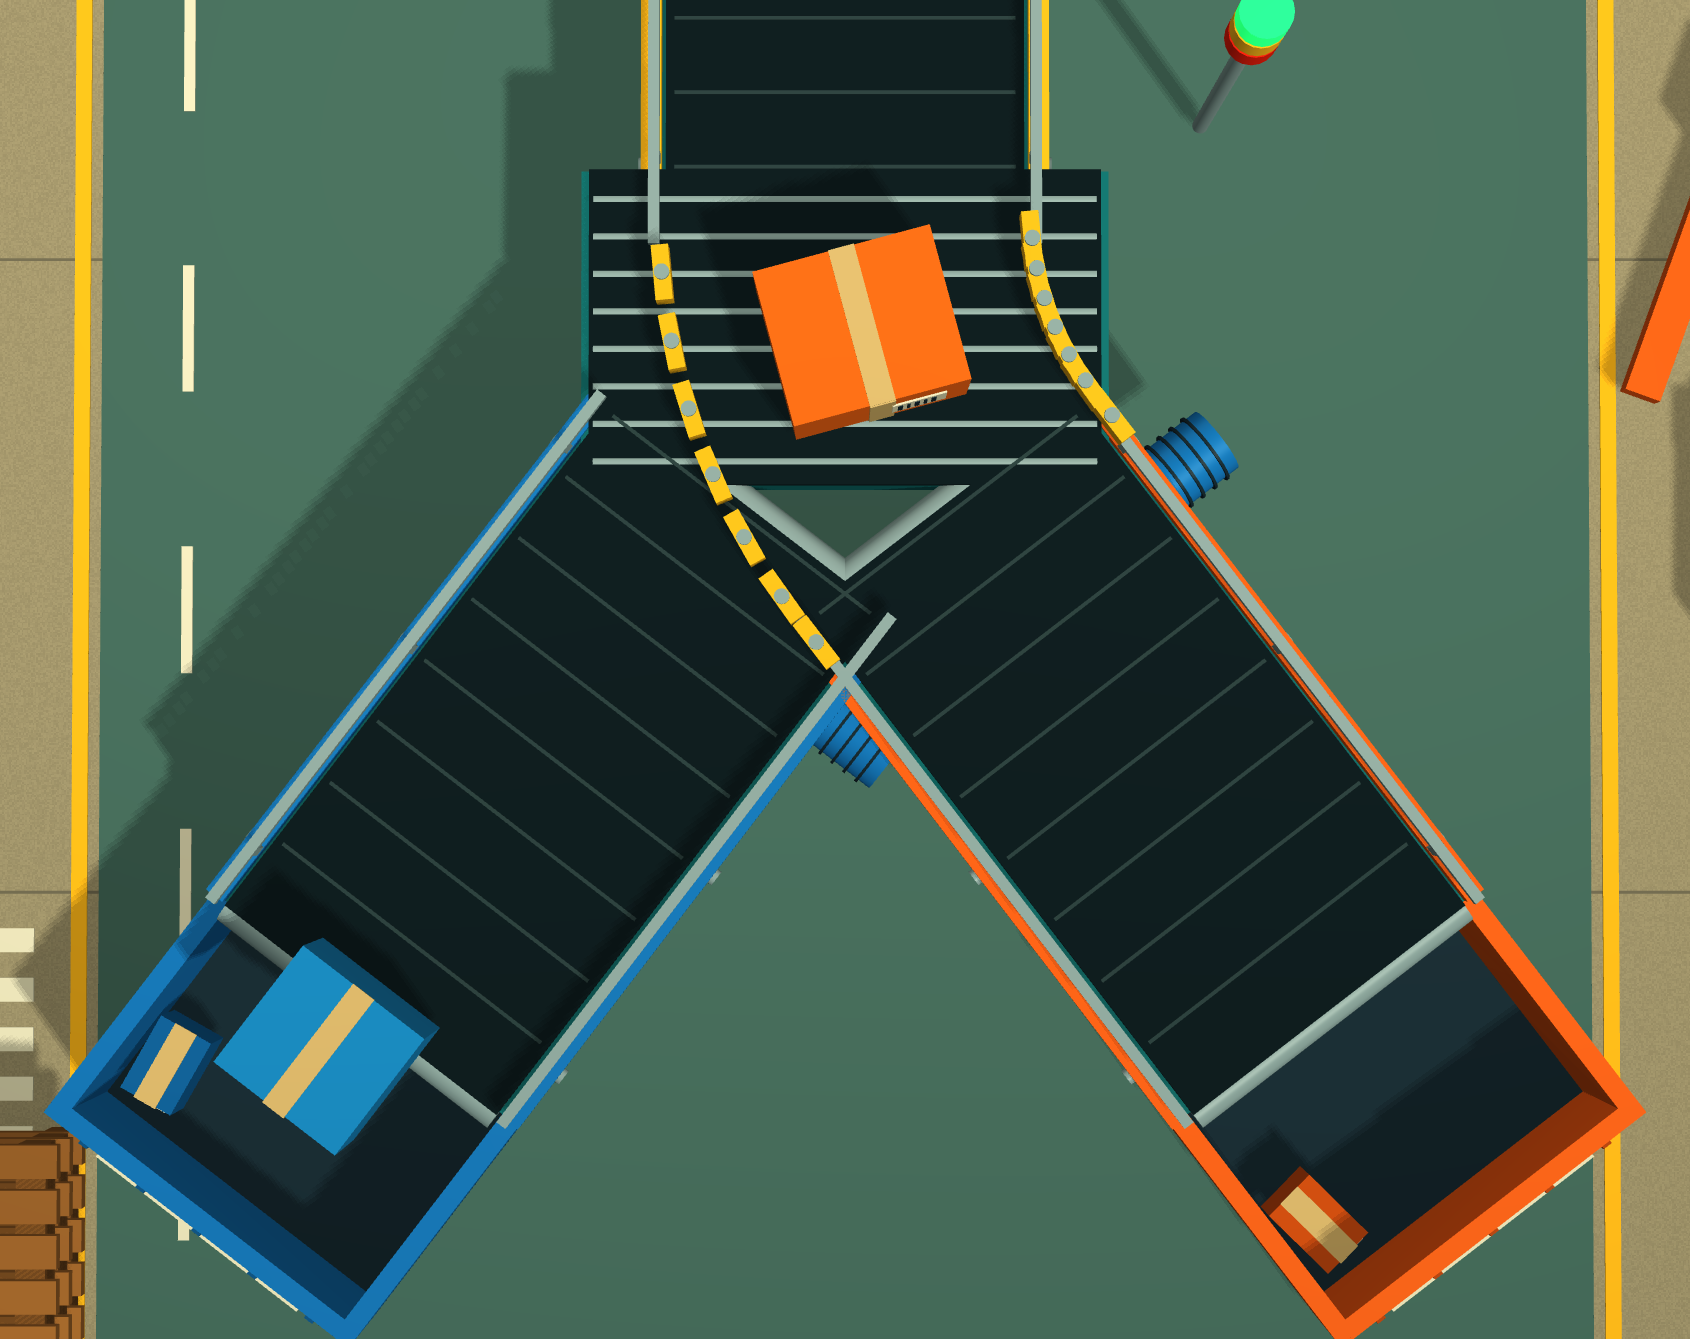
\includegraphics[width=\linewidth]{assets/gate_right_crop.png}\par\small\textbf{B. 12.25 s:} orange parcel starts the right route; gate $+37.5^\circ$.\end{minipage}
\caption{Matched overhead close-ups show the guide channel changing direction. Left and right refer to the machine's $x$ axis.}
\end{figure}
\subsection{Curved route model}
The first 1.80 units follow a circle, then the parcel follows a straight branch. Let $a=37.5^\circ$ in radians, $r=1.80/a\approx2.7502$, $s$ be route distance, $\sigma=-1$ for left or $+1$ for right, and $\beta=\operatorname{clamp}(s,0,1.80)/r$:
\begin{equation}
x=\sigma r(1-\cos\beta),\qquad z=r\sin\beta.
\end{equation}
These offsets start from $(0,1.55,4.00)$. After the arc, add $(\sigma\sin a,0,\cos a)\max(0,s-1.80)$. Center height is $1.55+h/2$. Yaw turns gradually as $\sigma37.5^\circ\operatorname{clamp}(s/1.80,0,1)$.
\begin{center}\begin{minipage}{0.67\linewidth}
\begin{shot}{assets/collection_crop.png}{At 13.15 s the first blue parcel has landed inside bin A. The recorded simulation state confirms Collected and counter A = 1.}
\callout{0.28,0.57}{0.19,0.81}{Collected blue box}
\callout{0.68,0.70}{0.80,0.88}{Exit belt}
\end{shot}
\end{minipage}\end{center}
\textbf{Collection and reuse:} the rear must clear the 5.50-unit route before dropping. Gravity lowers the box to $y=0.30+h/2$; its counter increases once. After 0.65 s the slot becomes free. A new parcel can spawn every 2.50 s when a slot and entry space are available. The 12-slot pool keeps the factory running without unlimited accumulation. One small static cargo box remains in each bin as decoration.
\source{\code{FactorySimulation.cpp}: \code{routePosition()}, \code{routeYaw()}, exit/drop/collection cases, \code{spawnBox()}.}
